\documentclass[main.tex]{subfiles}

\begin{document}

\section{Analisi e Ottimizzazione}\label{sec:ottimizzazione}
% incrociare tabelle della compute capabilities
% https://developer.nvidia.com/cuda-gpus#compute
% https://docs.nvidia.com/cuda/cuda-c-programming-guide/index.html#compute-capabilities


\subsection{Analisi delle prestazioni}
% è importante ottimizzare ma non bisogna andare alla cieca senno si perde tempo a fare qualcosa che magari occupa solo l'1% del tmempo totale. 
% messo su nsight system -> render occupa il 98% del tempo. è da ottimizzare

\hspace*{0.25in}Come ci insegna Donald Knuth \cite{knuth}, \textit{"le ottimizzazioni premature sono la radice di tutti i mali"}. Quindi, per evitare di procedere con ottimizzazioni guidate dal sentimento, è essenziale condurre un'analisi dettagliata dell'esecuzione del codice. 
Dopo aver scoperto che \textit{nvprof} è stato deprecato e che \textit{NVIDIA} ha deciso di non supportare la profilazione su \textit{WSL} (\textit{Windows Subsystem for Linux}, ambiente in cui lavoriamo entrambi), siamo in qualche modo riusciti a reperire un report. 
\begin{figure}[h]
    \centering
    \fbox{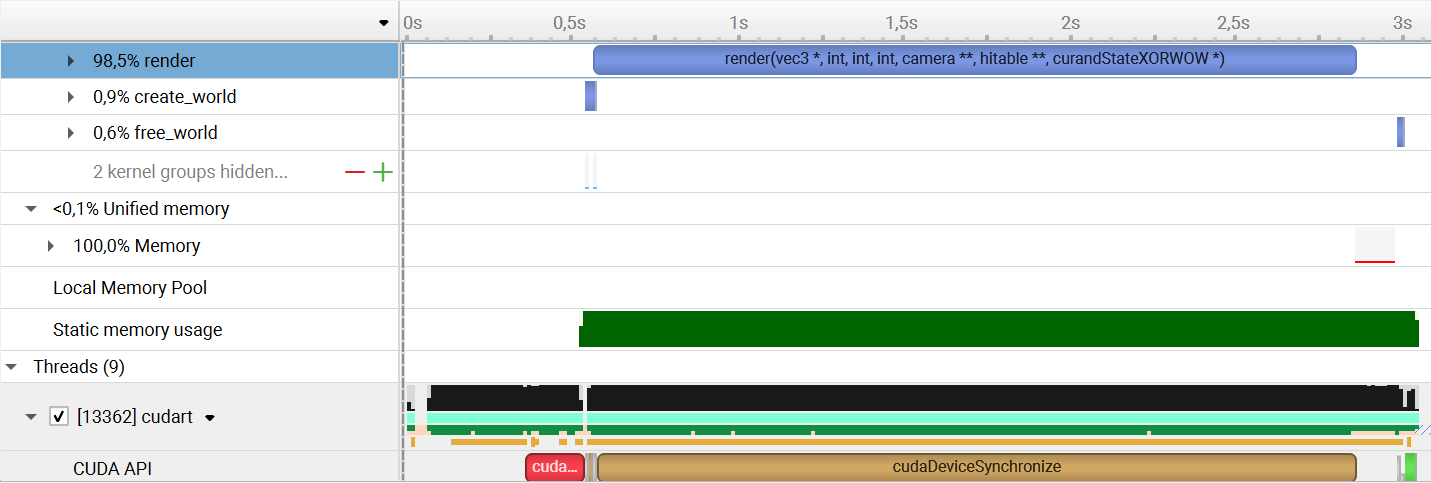
\includegraphics[width=0.9\textwidth]{figures/Analisys.png}}
    \captionsetup{aboveskip=0pt}
    \captionof{figure}{
    \centering
    Profilazione tramite Nsight System
    \hspace{1000pt}
    \small{N.B.: la profilazione è stata eseguita dopo l'ottimizzazione alle vtables, sezione 3.5.2}
    }\vspace{-14pt}\rule{0.95\linewidth}{0.4pt}
\end{figure}\\
Nella sezione iniziale, dedicata all'inizializzazione del profiler, emergono le fasi di allocazione della memoria, prima sull'\textit{host} (indicata in rosso tra le chiamate alle \textit{API CUDA}) e successivamente sul \textit{device} (evidenziata in blu tra le chiamate ai kernel).
Conforme alle aspettative, la stragrande maggioranza del tempo di esecuzione è attribuibile al kernel di rendering, rappresentando il 98,5\% dei tempi nei kernel e l'87,5\% del totale. Pertanto, è cruciale sviluppare strategie mirate a ridurre principalmente il tempo di esecuzione di questo componente.

\subsection{Dimensioni dei blocchi}
%grafico blocchi

% incrociare tabelle della compute capabilities per la gpu di toms 
% https://developer.nvidia.com/cuda-gpus#compute
% https://docs.nvidia.com/cuda/cuda-c-programming-guide/index.html#compute-capabilities
\hspace*{0.25in}Come prima cosa dobbiamo effettuare una scelta riguardo la dimensione dei blocchi da utilizzare per il kernel. Infatti, in base alle \textit{compute capabilities} della GPU, ci saranno 
% \vspace{100pt}
\begin{minipage}{0.6\textwidth}
\vspace{5pt}
 delle configurazioni che sfruttano meglio l'hardware del dispositivo. Questo dipende, inoltre, dall'utilizzo dei registri da parte dei thread del blocco e dalle operazioni che effettua in proporzione alle richieste in memoria: può accadere che il \textit{multi processor} non sia sfruttato a pieno, o che, al contrario, non abbia abbastanza risorse.
Inaspettatamente, la dimensione che genera il minor tempo di esecuzione è 32x32.
\end{minipage}%
\begin{minipage}{0.4\textwidth}
    \vspace{2pt}
    \centering
    \fbox{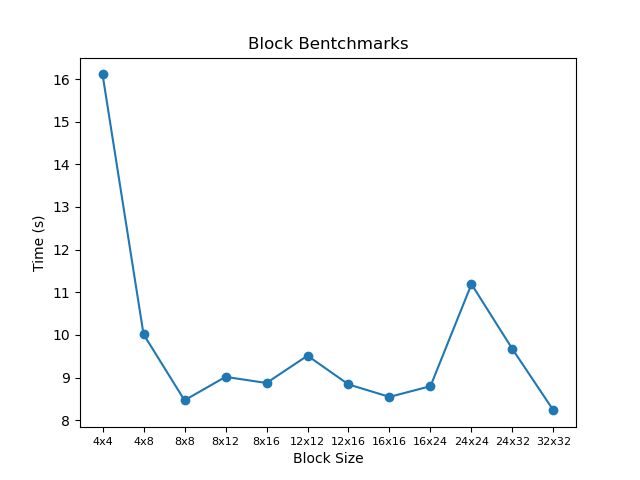
\includegraphics[width=0.8\textwidth]{figures/dim_plot.png}}
    \captionsetup{aboveskip=0pt}
    \captionof{figure}{Dimensioni dei Blocchi}\vspace{-14pt}\rule{1\linewidth}{0.4pt}
\end{minipage}\\


\subsection{Shared Memory}
% proviamo a velocizzare: notiamo che il tempo di esecuzione dipende molto dai sample utilizzati. i sample servono a definire meglio l'immagine per l'effetto antialiasing. possiamo dare un effetto simile utilizzando i sample dei pixel intorno piuttosto che far ripartire ogni volta nuovi sample.
% mettere img 32 sam no shm / 32 sam si shm / 50 sam no shm
% calcolo dello speed up

\hspace*{0.25in}Notiamo che il tempo di esecuzione dipende principalmente dal numero di oggetti nel mondo, con i quali i raggi devono calcolare l'intersezione minima, e dal numero di raggi emessi per campionare ogni pixel. Ci siamo concentrati soprattutto su quest'ultimo aspetto, attribuibile all'effetto anti-aliasing. \\
Come già accennato, lo svantaggio prestazionale degli algoritmi di ray tracing è dovuto alla scelta di trattare ogni raggio in modo separato, riavviando il processo di esecuzione ogni volta. Ma cosa accade se mettiamo in collaborazione pixel adiacenti?

L'idea è semplice: invece di far partire numerosi raggi da ciascun pixel, ne emettiamo pochi e sfruttiamo i risultati già calcolati dai pixel adiacenti. Per implementarla, sfruttiamo la \textit{shared memory}. \\
Ogni thread, corrispondente a un singolo pixel, si occupa di inizializzare la propria cella nella matrice condivisa. Successivamente, calcola la media dei colori restituiti dai raggi generati e la immagazzina nella sua cella di memoria. Solo quando tutti i thread 
\begin{minipage}{0.58\textwidth}
\vspace{12pt}
\begin{lstlisting}[style=cppstyle, label=cppexample]
__shared__ vec3	sh_mem[B_H][B_W];
... /* threads compute 'color' */ 
sh_mem[tIdx.y][tIdx.x] = color;
__syncthreads();
vec3 near_col = vec3(0,0,0);
near_col += sh_mem[tIdx.y][tIdx.x+1];
near_col += sh_mem[tIdx.y][tIdx.x-1];
near_col += sh_mem[tIdx.y+1][tIdx.x];
near_col += sh_mem[tIdx.y-1][tIdx.x];
color = (1-w)*color + w*near_col / 4;
\end{lstlisting}
\end{minipage}%
\hspace{10pt}
\begin{minipage}{0.39\textwidth}
   del blocco, che condividono la matrice, hanno completato il processo, inizia lo scambio di dati: ogni thread acquisisce i risultati dei pixel adiacenti dalla matrice e ne calcola la media. Infine, effettua una media ponderata tra il suo risultato e il calcolo appena effettuato, determinando il colore da assegnare al pixel.
\end{minipage} 
Si nota che un'immagine con circa 60 campioni è quasi indistinguibile da un'immagine con 25 campioni generata mediante l'approccio descritto. Inoltre, come previsto, la riduzione dei campioni da generare comporta una significativa diminuzione dei tempi di esecuzione.

\begin{figure}[h]
  \begin{minipage}{0.5\textwidth}
    \centering
    \fbox{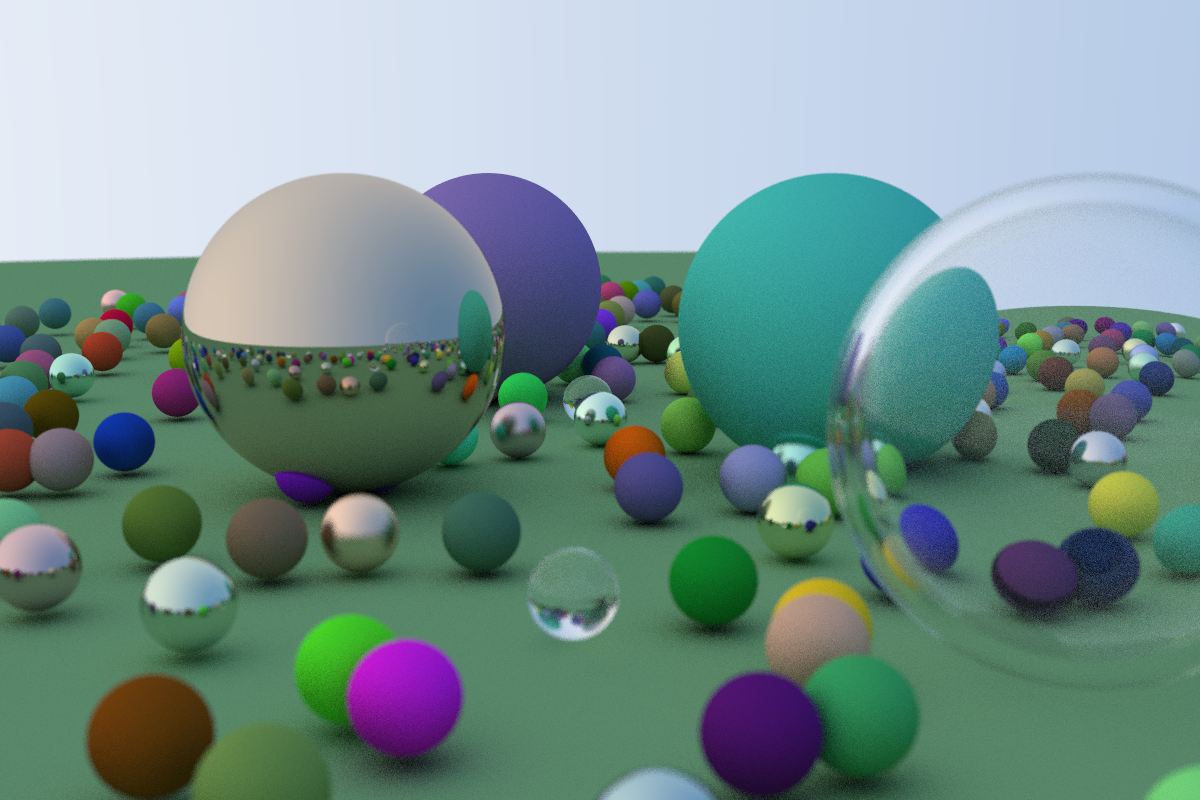
\includegraphics[width=0.9\linewidth]{figures/image_60.png}}
    \captionsetup{aboveskip=0pt}
    \captionof{figure}{
        \centering
        no Sh.Mem., 60 campioni. Tempo di esecuzione: 5.4s
    }\vspace{-14pt}\rule{0.85\linewidth}{0.4pt}

  \end{minipage}%
  \begin{minipage}{0.5\textwidth}
    \centering
    \fbox{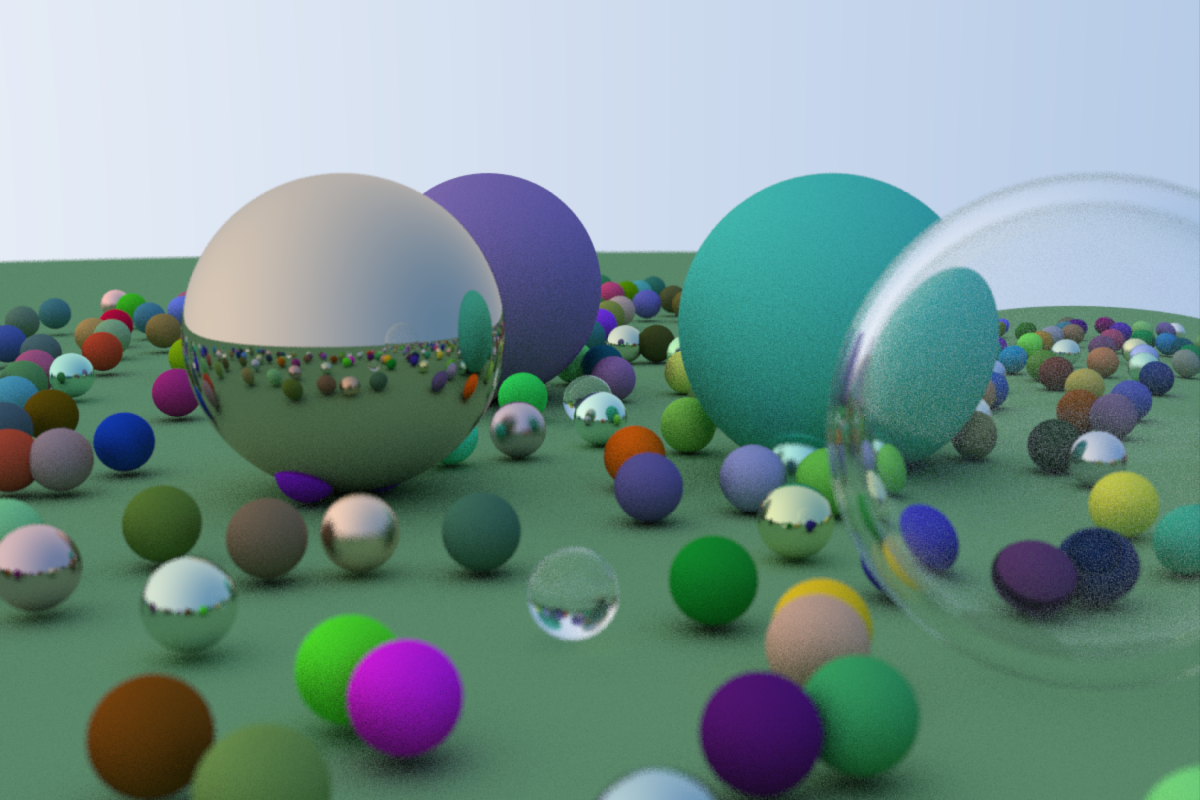
\includegraphics[width=0.9\linewidth]{figures/image_30_shared.png}}
    \captionsetup{aboveskip=0pt}
    \captionof{figure}{
        \centering
        con Sh.Mem., 30 campioni. Tempo di esecuzione: 2.7s        
    }\vspace{-14pt}\rule{0.85\linewidth}{0.4pt}
  \end{minipage}
\end{figure}

\subsection{Ottimizzazioni della Memoria}
% si nota dall'analisi che nella parte finale c'è un tempo significativo dedicato alla copia della memoria e ai page fault. e all'inizio c'è un tempo significativo (rosso) speso per la malloc managed. proviamo a risolverla con malloc host e memcpy piuttosto della unified memory
\hspace*{0.25in}Se torniamo all'analisi dell'esecuzione del programma, visibile in Figura 7, possiamo porre l'attenzione sul colore rosso, che in questo caso indica la memoria. La chiamata 
a funzione \textit{cudaMallocManaged} e i \textit{Page Fault} che si riscontrano a fine programma, evidenziati nella Figura 11, costituiscono il secondo evento più rilevante nell'analisi, occupando più del 10\% della totale esecuzione del programma. 
\begin{figure}[h]
    \centering
    \fbox{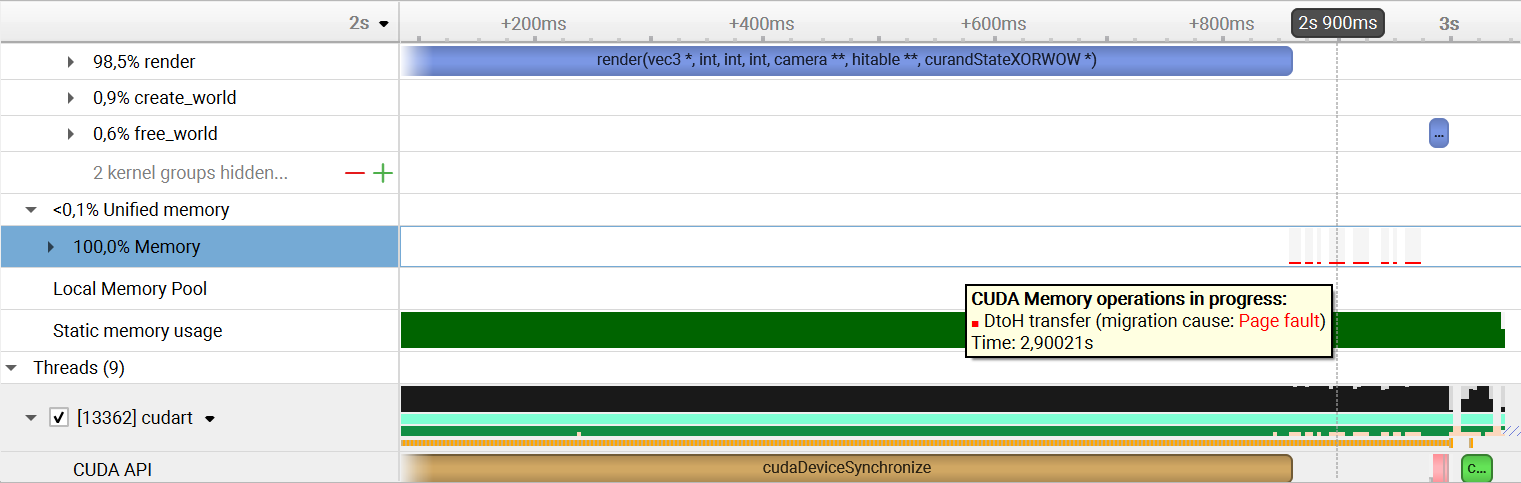
\includegraphics[width=0.9\textwidth]{figures/Analisys_memory.png}}
    \captionsetup{aboveskip=0pt}
    \captionof{figure}{Analisi della Memoria con Nsight System}\vspace{-14pt}\rule{0.65\linewidth}{0.4pt}
\end{figure}

Questo è dovuto all'utilizzo della cosiddetta \textit{Unified Memory}, che permette di mantenere la coerenza tra le memorie di \textit{host} e \textit{device} senza eseguire copie esplicite.
 Infatti, appena avviene una sincronizzazione al termine di un kernel, vengono riportate automaticamente le modifiche sulle memorie. Se da un lato facilita la scrittura di codice, dall'altro l'utilizzo della \textit{Unified Memory} può creare problemi prestazionali.  
Abbiamo deciso quindi di effettuare le copie in modo esplicito, sfruttando la funzione \textit{cudaMallocHost}, che permette di allocare i dati direttamente sulle pagine \textit{pinned}, e la funzione \textit{cudaMemcpy}. 

\begin{lstlisting} [style=cppstyle, label=cppexample]
// cudaMallocManaged((void **)&d_buf, BSIZE);
cudaMallocHost((void **)&h_buf, BSIZE));
cudaMalloc((void **)&d_buf, BSIZE));
cudaMemcpy(d_buf, h_buf, BSIZE, cudaMemcpyHostToDevice));
... /* kernel di rendering */
cudaMemcpy(h_buf, d_buf, BSIZE, cudaMemcpyDeviceToHost);
\end{lstlisting}

% TODO (Forse): da mettere cosa abbiamo ottenuto?

% sempre riguardo a memcpy, possiamo provare a togliere del lavoro alla gpu creando il mondo sulla cpu (migliore per i lavori sequenziali). si creano però dei problemi di dipendenza tra classi che rendono impossibile quanto detto
Nonostante la creazione del mondo non costituisca un problema dal lato delle prestazioni, abbiamo voluto provare un approccio diverso per avere il controllo del mondo anche lato \textit{host}. In particolare, abbiamo provato ad allocare gli oggetti prima sull'\textit{host}, per poi copiarli sul \textit{device}. Avendo una lista di oggetti, abbiamo provato a seguire il pattern della copia di \textit{Array of Struct}, con l'idea di migliorarla successivamente con il pattern di \textit{Array of Struct}. Ci siamo accorti, però, che gli oggetti utilizzati sono ben più complessi di semplici strutture dati. Infatti, i dati che contengono sono spesso puntatori ad oggetti di altre classi, andando a formare una catena di dipendenze difficile da sciogliere. 

\subsection{Ottimizzazioni Generali}
% get_color() iterativo invece di ricorsivo
%v_table
\hspace*{0.25in}Per migliorare ulteriormente le prestazioni, possiamo ridurre alcune operazioni che risultano essere computazionalmente onerose, come l'utilizzo di funzioni ricorsive, il recupero delle \textit{VTables} (\textit{Virtual Tables}) delle classi e l'eccessiva precisione nei calcoli. 

\subsubsection{Funzioni ricorsive}
La funzione responsabile di calcolare il colore per un raggio è stata implementata inizialmente in modo ricorsivo per migliorare la comprensione del codice. La funzione si occupava di calcolare il punto d'intersezione e la nuova direzione del raggio, per poi chiamarsi ricorsivamente utilizzando i parametri appena calcolati. Lo stesso risultato è stato raggiunto attraverso l'utilizzo di un'analoga funzione iterativa.

\subsubsection{Recupero delle Virtual Tables delle classi}
Il recupero delle \textit{VTables} è demandato alla risoluzione della chiamata a funzione in fase di runtime, anziché al compilatore. Questo processo può essere considerato lento soprattutto in base all'utilizzo delle classi nel codice. Nel nostro contesto, le funzioni critiche sono principalmente quelle dedicate al \textit{sampling} e al calcolo delle collisioni. Pertanto, abbiamo introdotto varianti delle funzioni originali, strutturate in modo tale da non appartenere a classi. \\
Questa scelta ci ha permesso di ottenere notevoli miglioramenti nei tempi di esecuzione, ma non è stata estesa a tutte le situazioni: ad esempio, nella diffusione dei materiali, riprodurre l'ottimizzazione avrebbe implicato di dover effettuare diversi controlli per selezionare la corretta funzione da chiamare; abbiamo quindi deciso di non farlo. 
C'è da sottolineare che, mentre questa operazione di ottimizzazione può essere estremamente efficace in determinate situazioni, potrebbe rivelarsi altrettanto inefficace in altre, a seconda delle caratteristiche specifiche di implementazione e utilizzo nel codice.

\subsubsection{Precisione dei Calcoli}
%fast_math: leggi la documentazione
Le moderne GPU raggiungono le massime prestazioni quando eseguono calcoli in precisione singola, mentre i calcoli a doppia precisione possono risultare notevolmente più lenti. Pertanto, è cruciale fare attenzione durante la costruzione di espressioni con numeri decimali: è sempre buona pratica aggiungere il suffisso \textit{'f'} per evitare che il compilatore interpreti il dato come un numero \textit{double}. \\
Inoltre, è possibile sacrificare ulteriormente la precisione dei calcoli abilitando in fase di compilazione l'utilizzo delle librerie di \textit{fast math} tramite il \textit{flag} dedicato. Questa rende le operazioni di addizione, moltiplicazione, divisione e radice quadrata molto più veloci, approssimandone i risultati. Non abbiamo notato una visibile perdita nella qualità dell'immagine generata.


\subsection{Limiti: Warp Divergence}
% è un problema noto. link ai paper.
\hspace*{0.25in}La divergenza del warp si manifesta quando i thread all'interno di un warp intraprendono percorsi di esecuzione diversi a causa di costrutti di controllo condizionale, come istruzioni \textit{if} o \textit{switch}. Questi thread sono vincolati a seguire il medesimo flusso di codice, per cui, anche se solo uno di essi si immette in una branca condizionale, tutti gli altri sono costretti a seguirla e ad attendere il suo completamento.\\
La divergenza rappresenta un noto problema nel contesto del Ray Tracing \cite{divergence}, poiché costituisce una caratteristica intrinseca del comportamento dei raggi. La casualità associata alle riflessioni e rifrazioni genera spesso situazioni di divergenza, soprattutto nei pressi dei contorni degli oggetti, in cui alcuni raggi vengono diffusi mentre altri no.\\
La \textit{Warp Divergence} incide negativamente sulle prestazioni complessive del Ray Tracer in quanto comporta una sottoutilizzazione delle risorse della GPU. Tuttavia, essa ha contribuito nello sviluppo di nuovi algoritmi innovativi incitando la ricerca di nuove idee e l'utilizzo di nuove tecnologie per ovviare al problema.

\subsection{Possibili Soluzioni: Dynamic Parallelism e Blocchi 3D }
% per continuare l'ottimizzazione abbiamo provato a parallelizzare il kernel tramite il dyn-par. chiedi a tommaso
\hspace*{0.25in}Un approccio per mitigare la divergenza dei warp consiste nell'utilizzo della parallelizzazione dinamica, che comporta il lancio di kernel, detti figli, a partire da altri kernel, detti padre. Questo approccio, nel nostro contesto, si può applicare alla fase di rendering: ogni thread lancia un nuovo kernel in modo che ognuno dei thread figli sia responsabile della computazione di un singolo campione.\\
In primo luogo, si verifica un notevole aumento del numero di thread schedulati, che si traduce sì in maggior parallelizzazione, ma anche in maggior overhead di schedulazione. In secondo luogo, emerge un problema di sincronizzazione, poiché è necessario raccogliere tutti i risultati per poter di procedere. Dato che i kernel sono di base asincroni, per fare questo è richiesta una sincronizzazione manuale, deprecata e quindi da forzare in fase di compilazione tramite la flag \textit{-DCUDA\_FORCE\_CDP1\_IF\_SUPPORTED} \cite{man}. Tuttavia, questo approccio comporta uno stress eccessivo sulla GPU, causando un rallentamento significativo rispetto ai metodi precedenti dovuto continue sincronizzazioni.

Un secondo metodo per ridurre la divergenza dei warp consiste nella pianificazione di blocchi tridimensionali, che considerano il numero di campioni come grandezza aggiuntiva. Ciò consente di ridurre notevolmente i costi di sincronizzazione, ma fa sorgere due nuovi problemi: primo, deve essere presente un thread master per ogni pixel che si occupi di riunire i dati restituiti dagli altri e questo genera divergenza; secondo, il numero di campioni è limitato dalle \textit{compute capabilities} della GPU, le quali stabiliscono un massimo di 1024 thread per blocco.\\
In definitiva, pur ottenendo un lieve aumento delle prestazioni, il costo associato a questo approccio risulta comunque più elevato rispetto alle tecniche descritte nelle sezioni precedenti.


\end{document}